\section{Abstract Syntax Tree en Golang}
\textit{Golang} provee una serie de paquetes que permiten trabajar con código fuente escrito en ese lenguaje de programación, facilitando la creación de \textbf{árboles de sintáxis abstracta}, para el análisis o manipulación de los mismos.
Al ser provisto oficialmente por los creadores, no es necesario definir la gramática para alguna otra herramienta como ANTLR.
Además, esto nos asegura que se soportan todas las estructuras que componen el lenguaje y se encuentran definidas en la especificación del mismo [AGREGAR REFERENCIA].

\begin{figure}[H]
  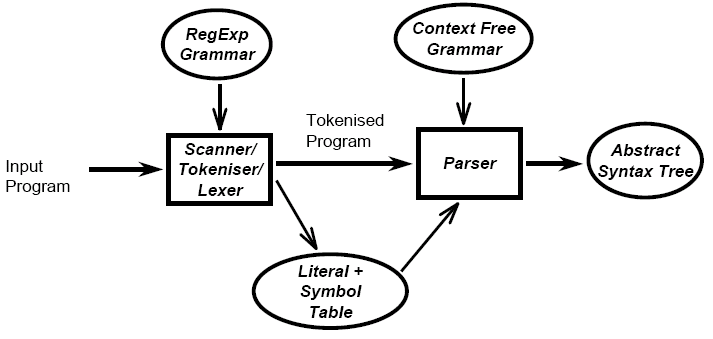
\includegraphics[width=12cm]{implementation/parsingpipeline}
  \centering
  \caption{Creación de un AST desde código fuente}
\end{figure}

En la figura X se establece la correlación entre las etapas del proceso de creación de un AST a partir de código fuente y los paquetes provistos en el lenguaje de programación.
La función de cada uno de estos, y su participación en el proceso, se indica a continuación:
\begin{itemize}
  \item \textbf{go/token} Contiene... TODO
  
  \item \textbf{go/scanner} TODO
  
  \item \textbf{go/ast} TODO
  
  \item \textbf{go/parser} El paquete contiene las funciones y estructuras necesarias para el parseo de archivos Go, los cuales se pueden prover de diferentes formas (por archivo, directorio, etc).
  El resultado del parseo es el árbol de sintáxis abstracta (AST), el cual puede luego ser procesado para evaluar, extraer información e incluso modificarlo.
  Las funciones y configuraciones principales de este paquete son:
  \begin{itemize}
    \item \textbf{ParseFile(fset *token.FileSet, filename string, src interface{}, mode Mode) (f *ast.File, err error)} Esta función realiza el parseo de un sólo archivo de Go y retorna el nodo correspondiente a \textbf{ast.File}. El elemento retornado solamente representa el archivo en cuestión, sin tener en cuenta los demás elementos del paquete/proyecto, por lo que es necesario armar el árbol completo con los resultados de cada una de sus llamadas.
    
    VER qué más de acá: ParseFile parses the source code of a single Go source file and returns the corresponding ast.File node. The source code may be provided via the filename of the source file, or via the src parameter. If src != nil, ParseFile parses the source from src and the filename is only used when recording position information. The type of the argument for the src parameter must be string, []byte, or io.Reader. If src == nil, ParseFile parses the file specified by filename. The mode parameter controls the amount of source text parsed and other optional parser functionality. Position information is recorded in the file set fset, which must not be nil. If the source couldn't be read, the returned AST is nil and the error indicates the specific failure. If the source was read but syntax errors were found, the result is a partial AST (with ast.Bad* nodes representing the fragments of erroneous source code). Multiple errors are returned via a scanner.ErrorList which is sorted by file position.

    \item \textbf{Mode}
    
  \end{itemize}
  
\end{itemize}
